\documentclass[main.tex]{subfiles}
\newlength{\retraittableau}
\setlength{\retraittableau}{-4mm}
\newlength{\firstcolwidth} %% on ne peut mettre ni chiffre ni caractere special dans le nom d'une longueur
\setlength{\firstcolwidth}{22mm}
\begin{document}
\chapter{Optimisation de la reconstruction d'image scanner}
\lettrine[lines=2, lhang=0.33, loversize=0.25]{M}{aintenant} que nous avons un modèle EDP qui reproduit bien les aspects constatés en clinique, interrogeons nous sur la manière de reconstruire une image en niveau de gris (image scanner) à partir des résultats numériques \ie de l'évolution des densités $N(t,x)$, $P(t,x)$ et $S(t,x)$ (toutes comprises entre 0 et 1). On tentera, dans ce chapitre, d'optimiser les niveaux de gris $\tau_N, \tau_P$ et $\tau_S$ de l'interpolation EQREF \todo[noline]{eqref} afin de rapprocher au maximum la visualisation des résultas numériques de la visualisation des scanners médicaux.

\section{Présentation de l'approche}
Pour un patient donné, on considère $n$ instants auxquels on possède des scanners (aux temps $t_i, i\in \{ 1,...,n \}$). Sur ces $n$ images, on propose d'optimiser les coefficients de l'interpolation $\tau_N N + \tau_P P + \tau_S S$:
\begin{equation}
\begin{aligned}
\frac{1}{\aire\big(Z_1(t_i)\big)}&\left( \tau_N\intperso{Z_1(t_i)}N(t_i,x) \dx + \tau_P\intperso{Z_1(t_i)}P(t_i,x) \dx + \tau_S\intperso{Z_1(t_i)} S(t_i,x) \dx \right) \\
&= \frac{1}{\aire\big(Z_2(t_i)\big)} \ \intperso{Z_2(t_i)} s(t_i,x,z_0) \dx \qquad i \in \{1,...,n\}
\end{aligned}
\end{equation}
où : \begin{itemize}
\item $\aire(Z)$ est l'aire de la zone $Z$.
\item $Z_1(t_i)$ est la zone correspondant à la tumeur dans les simulations numériques au temps $t_i$. Elle est définie par un seuillage sur $S$.
\todo[noline]{specifier le seuillage ?}
\item $Z_2(t_i)$ est la zone tumorale sur le scanner réalisé au temps $t_i$. Cette zone a été définie par contourage manuel à l'aide du logiciel OsiriX.
\item $z_0$ est la coupe que l'on choisie d'étudier dans les scanners. Cette coupe est approximativement la même au cours du temps.
\item $s(t_i,x,z_0)$ est la valeur du niveaux de gris du pixel en position $x$ sur la coupe $z_0$ du scanner effectué au temps $t_i$.
\end{itemize}
En utilisant la discrétisation, aussi bien sur les simulations numériques que sur les scanners, on obtient :
\begin{equation}
\begin{aligned}
\frac{1}{\mathcal{N}\big(Z_1(t_i)\big)}&\left( \tau_N\!\!\sum_{x\in Z_1(t_i)}\!\!N(t_i,x) + \tau_P\!\!\sum_{x\in Z_1(t_i)}\!\!P(t_i,x) + \tau_S\!\!\sum_{x\in Z_1(t_i)}\!\!S(t_i,x) \right) \\
&= \frac{1}{\mathcal{N}\big(Z_2(t_i)\big)} \sum_{x\in Z_2(t_i)}\!\! s(t_i,x,z_0) \qquad i \in \{1,...,n\}
\end{aligned}
\end{equation}
où $\mathcal{N}(Z)$ désigne le nombre de pixel contenu dans la zone $Z$. On a donc un système linéaire de 3 inconnues à $n$ équations que l'on peut réécrire :
\begin{equation}
A\tau=B,
\end{equation}
avec $\tau= \trans(\tau_N,\tau_P,\tau_S)$, $A$ matrice de taille $n\times 3$ et $B$ vecteur colonne de taille $n$.

Pour ne pas se limiter au cas $n=3$ qui clos le système, on le résoud par la minimisation suivante :
\begin{equation}\label{eq:min_optim_grey}
\min_{\tau} \left( \dfrac{\| A\tau - B \|^2_{\ell^2}}{\|B\|^2_{\ell^2}} + \mathcal{P}(\tau) \right),
\end{equation}
où la pénalisation $\mathcal{P}$ permet d'assurer que les optima respectent les bornes~0 à~255 :
\begin{equation}
\label{eq:penalisation_creneau}
\mathcal{P}(\tau) = 1e7 \times ( \tau \notin  [0;255]^3 ).
\end{equation}

\section{Optimisation sur 3 paramètres}
%\DTLloaddb{optim3_0grey}{../data/cout_1/optim3.csv}
%\DTLloaddb[noheader]{optim3_0leg}{../data/cout_1/optim3_leg.csv}
%\DTLloaddb{optim3_0stat}{../data/cout_1/optim3_stat.csv}
%%\DTLloaddb[noheader]{optim3_0stat}{../data/cout_1/optim3_stat.csv}
%%\DTLsetheader{optim3_0stat}{Column1}{}
%\DTLsetheader{optim3_0leg}{Column1}{}
%\DTLsetheader{optim3_0leg}{Column2}{}
%\begin{sidewaystable}
%\footnotesize\smaller[0.5]
%%\scriptsize
%\centering
%\begin{tabular}{|c|c|c|c|c|}
%\hline
%%%\hhline{|>{\arrayrulecolor{white}}->{\arrayrulecolor{black}}|-|-|}
%\rowcolor{gray!70}
%& \multicolumn{4}{c|}{ \cellcolor{gray!70} \bfseries  Algorithme d'optimisation} \\
%\hhline{|>{\arrayrulecolor{gray!70}}->{\arrayrulecolor{black}}|-|-|-|-|}
%\rowcolor{gray!70}
%& \bfseries SLSQP
%& \bfseries GC 
%& \bfseries Neldear-Mead 
%& \bfseries BFGS \\
%\rowcolor{gray!70}
%\multirow{-3}{\firstcolwidth}{\scriptsize \bfseries \centering Scanners choisis pour l'optimisation}
%& $\tau_N, \qquad \tau_P, \qquad \tau_S$
%& $\tau_N, \qquad \tau_P, \qquad \tau_S$
%& $\tau_N, \qquad \tau_P, \qquad \tau_S$
%& $\tau_N, \qquad \tau_P, \qquad \tau_S$
%%%\\ \hline &&
%%%\\ \multicolumn{3}{|c|}{\rule{3cm}{1pt}}
%\DTLforeach*{optim3_0grey}{%
%\scan=scan,\NM=NM,\BFGS=BFGS,\col=SLSQP,\CG=CG,
%\errNM=errNM,\errBFGS=errBFGS,\errcol=errSLSQP,\errCG=errCG}{%
%\\
%\DTLifoddrow{\rowcolor{white}}{\rowcolor{gray!40}}%
%\scan & \begin{tabular}{c}
%\col \\ \errcol
%\end{tabular} & \begin{tabular}{c}
%\CG \\ \errCG
%\end{tabular} & \begin{tabular}{c}
%\NM \\ \errNM
%\end{tabular} & \begin{tabular}{c}
%\BFGS \\ \errBFGS
%\end{tabular} 
%}%
%\DTLforeach*{optim3_0stat}{%
%\NM=NM,\BFGS=BFGS,\col=SLSQP,\CG=CG}{%
%\\ \hline \hline %\DTLifoddrow{\rowcolor{white}}{\rowcolor{gray!40}}%
%Moyenne : & \col & \CG & \NM & \BFGS  }
%\\ \hline
%\end{tabular}
%\caption{\label{tab:optim3gris} Tableau récapitulatif des optimisations pour les 3 niveaux de gris}
%\end{sidewaystable}
%\DTLcleardb{optim3_0leg}
%\DTLcleardb{optim3_0stat}
%\DTLcleardb{optim3_0stat}


\DTLloaddb{optim3_0grey}{../data/cout_1/optim3.csv}
\DTLloaddb[noheader]{optim3_0leg}{../data/cout_1/optim3_leg.csv}
\DTLloaddb{optim3_0stat}{../data/cout_1/optim3_stat.csv}
%\DTLloaddb[noheader]{optim3_0stat}{../data/cout_1/optim3_stat.csv}
%\DTLsetheader{optim3_0stat}{Column1}{}
\DTLsetheader{optim3_0leg}{Column1}{}
\DTLsetheader{optim3_0leg}{Column2}{}
\begin{sidewaystable}
\footnotesize\smaller[0.5]
%\scriptsize
\centering
\begin{tabular}{|c|c|c|c|c|}
\hline
%%\hhline{|>{\arrayrulecolor{white}}->{\arrayrulecolor{black}}|-|-|}
\rowcolor{gray!70}
& \multicolumn{4}{c|}{ \cellcolor{gray!70} \bfseries  Algorithme d'optimisation} \\
\hhline{|>{\arrayrulecolor{gray!70}}->{\arrayrulecolor{black}}|-|-|-|-|}
\rowcolor{gray!70}
& \bfseries SLSQP
& \bfseries GC 
& \bfseries Neldear-Mead 
& \bfseries BFGS \\
\rowcolor{gray!70}
\multirow{-3}{\firstcolwidth}{\scriptsize \bfseries \centering Scanners choisis pour l'optimisation}
& $\tau_N, \qquad \tau_P, \qquad \tau_S$
& $\tau_N, \qquad \tau_P, \qquad \tau_S$
& $\tau_N, \qquad \tau_P, \qquad \tau_S$
& $\tau_N, \qquad \tau_P, \qquad \tau_S$
%%\\ \hline &&
%%\\ \multicolumn{3}{|c|}{\rule{3cm}{1pt}}
\DTLforeach*{optim3_0grey}{%
\scan=scan,\NM=NM,\BFGS=BFGS,\col=SLSQP,\CG=CG,
\errNM=errNM,\errBFGS=errBFGS,\errcol=errSLSQP,\errCG=errCG}{%
\\
\DTLifoddrow{\rowcolor{white}}{\rowcolor{gray!40}}%
\scan & \begin{tabular}{c}
\col \\ \errcol
\end{tabular} & \begin{tabular}{c}
\CG \\ \errCG
\end{tabular} & \begin{tabular}{c}
\NM \\ \errNM
\end{tabular} & \begin{tabular}{c}
\BFGS \\ \errBFGS
\end{tabular} 
}%
\DTLforeach*{optim3_0stat}{%
\NM=NM,\BFGS=BFGS,\col=SLSQP,\CG=CG}{%
\\ \hline \hline %\DTLifoddrow{\rowcolor{white}}{\rowcolor{gray!40}}%
Moyenne : & \col & \CG & \NM & \BFGS  }
\\ \hline
\end{tabular}
\caption{\label{tab:optim3gris} Tableau récapitulatif des optimisations pour les 3 niveaux de gris}
\end{sidewaystable}
\DTLcleardb{optim3_0leg}
\DTLcleardb{optim3_0stat}
\DTLcleardb{optim3_0stat}
La résolution de l'équation~\eqref{eq:min_optim_grey} fournit donc le $\tau$ optimal. Examinons les différences lorsque l'on fait varier :
\begin{itemize}
\item le nombre d'images considérées
\item les moments considérés
\item l'algorithme d'optimisation lui-même
\item la fonction coût utilisée
\end{itemize}

Dans tous les cas, on ne considèrera pas le premier scanner (numéro~0) car la condition initiale numérique EQREF \todo[noline]{EQREF} n'est pas prise de sorte à respecter la répartition des niveaux de gris du scanner. Evitons donc d'inclure dans l'optimisation une erreur de base qui serait incompressible.
\todo[noline]{Presenter numerotation des scans}


La Table~\ref{tab:optim3gris} synthétise l'ensemble des résultats d'optimisation obtenus sur les différents tests qui ont été réalisés. 
On remarque que plus le nombre d'image considérées est grand, plus l'erreur à convergence est grande. Ce comportement est attendu et ne pose pas de problème tant que l'erreur reste acceptable (de l'ordre de quelques pourcents). Augmenter le nombre d'images considérées s'avère utile pour rendre les optima moins sensibles aux perturbations éventuelles qu'il y a sur les données (bruit, marge d'erreur de segmentation manuelle, etc ...).


On peut de plus remarquer que selon les images choisies et selon les algorithmes choisis les résultats sont assez variables. Les moyennes des optima trouvés selon l'algorithme sont présentés sur la dernière ligne de la Table~\ref{tab:optim3gris}. Seul l'algorithme SLSQP se démarque des autres qui ont une valeur moyenne de $\tau_P$ non seulement proche de $\tau_S$ - ce qui ne facilite pas du tout le contraste du tissu proliférant avec le tissu sain - mais aussi supérieur à $\tau_S$ alors qu'on s'attendrait plutôt à l'inverse...
\todo[inline]{ FAUX !!! \\
En fait le paramètre $\tau_S$ est très peu influent dans le calcul de l'erreur~\eqref{eq:min_optim_grey} car il n'y a que très peu de tissu sain dans le périmètre tumoral. La valeur de $\tau_S$ n'a donc que très peu de poids et donc il est difficile de la déterminer avec ce type d'approche.
}

On note également que la combinaison $[1,9,11]$ ne semble pas pertinente pour calculer les niveaux de gris puisque les optima tendent vers les bornes autorisées ($[0,255]$).

%%%%%  ---- SECTION  OPTIM SUR 2 NVX DE GRIS ----- %%%%%
\section{Optimisation sur 2 paramètres, $\tau_S$ fixé}
Pour essayer de palier aux problèmes rencontrés dans la section précédentes, nous allons fixer $\tau_S$ à une valeur de 197 (sur l'échelle des niveaux de gris de 0 à 255). Cette valeur a été fixée en réalisant un contourage d'une zone en tissu sain dans OsiriX (cf. Figure~\ref{fig:contourage_sain}). La moyenne de ce contourage est de 134.5 HU. Le niveau de gris étant échelonné linéairement entre~-135 et~215, on peut ainsi faire correspondre cette quantité en HU à un niveau de gris compris entre~0 et~255. Ainsi, selon l'échelle considérée ici, 134.5~HU équivaut à un gris de 77\% soit un gris de niveau~197.
\todo[inline]{schema correspondance HU \% et grey lvl}

\begin{figure}
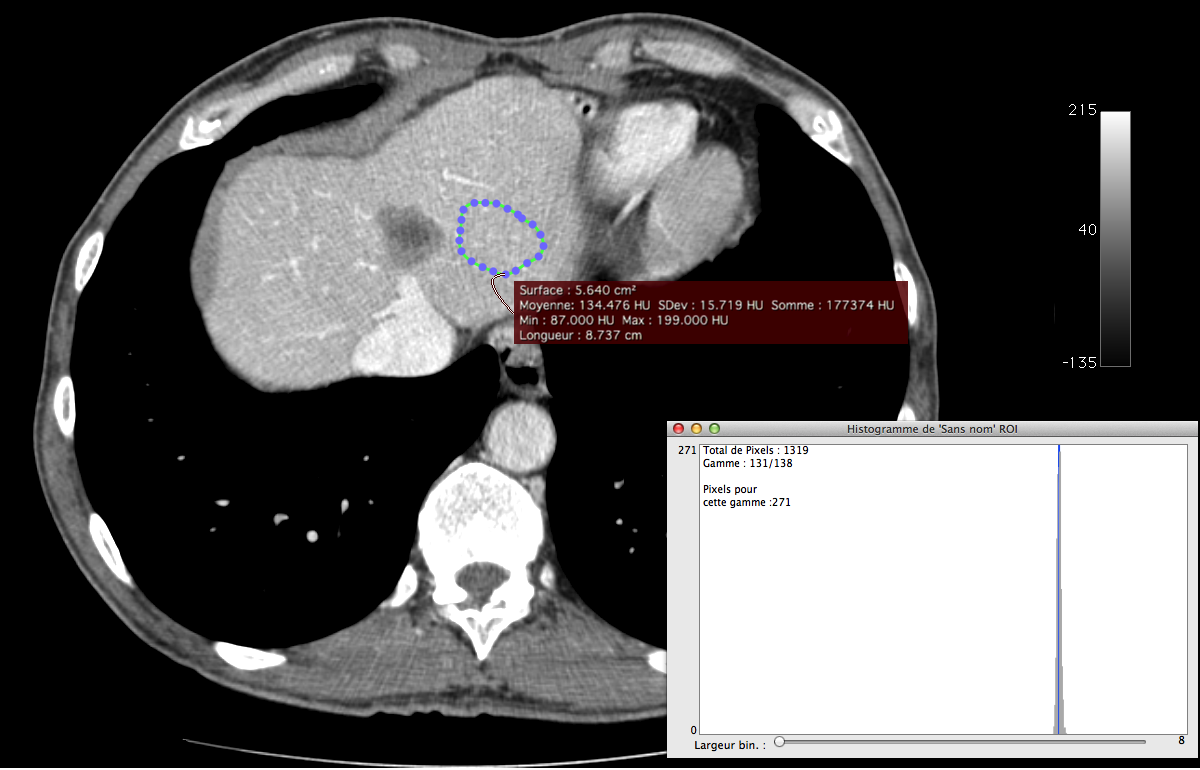
\includegraphics[width=\textwidth]{OsiriX_gris_sain_rognee.png}
\caption{\label{fig:contourage_sain}Contourage d'une zone saine -- Moyenne de la valeur des pixels dans ce périmètre : 134.5 HU (avec une échelle HU de \mbox{-135 à 215}).}
\end{figure}

%%%%%%% Cout0
%\DTLloaddb{optim2_0grey}{../data/cout_0/optim2.csv}
%\DTLloaddb[noheader]{optim2_0leg}{../data/cout_0/optim2_leg.csv}
%\DTLloaddb{optim2_0stat}{../data/cout_0/optim2_stat.csv}
%\DTLsetheader{optim2_0leg}{Column1}{}
%\DTLsetheader{optim2_0leg}{Column2}{}
%\begin{table}[htbp]
%\footnotesize
%\hspace{\retraittableau} %%% Le tableau depasse sur les marges !
%\begin{tabular}{|c|c|c|c|c|}
%\hline
%%%\hhline{|>{\arrayrulecolor{white}}->{\arrayrulecolor{black}}|-|-|}
%\rowcolor{gray!70}
%& \multicolumn{4}{c|}{ \cellcolor{gray!70} \bfseries  Algorithme d'optimisation} \\
%\hhline{|>{\arrayrulecolor{gray!70}}->{\arrayrulecolor{black}}|-|-|-|-|}
%\rowcolor{gray!70}
%& \bfseries SLSQP
%& \bfseries GC 
%& \bfseries Neldear-Mead 
%& \bfseries BFGS \\
%\rowcolor{gray!70}
%\multirow{-3}{\firstcolwidth}{\scriptsize \bfseries \centering Scanners choisis pour l'optimisation}
%& $\tau_N, \qquad \tau_P$
%& $\tau_N, \qquad \tau_P$
%& $\tau_N, \qquad \tau_P$
%& $\tau_N, \qquad \tau_P$
%\DTLforeach*{optim2_0grey}{%
%\scan=scan,\NM=NM,\BFGS=BFGS,\col=SLSQP,\CG=CG,
%\errNM=errNM,\errBFGS=errBFGS,\errcol=errSLSQP,\errCG=errCG}{%
%\\
%\DTLifoddrow{\rowcolor{white}}{\rowcolor{gray!40}}%
%\scan & \begin{tabular}{c}
%\col \\ \errcol
%\end{tabular} & \begin{tabular}{c}
%\CG \\ \errCG
%\end{tabular} & \begin{tabular}{c}
%\NM \\ \errNM
%\end{tabular} & \begin{tabular}{c}
%\BFGS \\ \errBFGS
%\end{tabular} 
%}%
%\DTLforeach*{optim2_0stat}{%
%\NM=NM,\BFGS=BFGS,\col=SLSQP,\CG=CG}{%
%\\ \hline \hline %\DTLifoddrow{\rowcolor{white}}{\rowcolor{gray!40}}%
%Moyenne : & \col & \CG & \NM & \BFGS  }
%\\ \hline
%\end{tabular}
%\caption{\label{tab:optim2gris0}Tableau récapitulatif des optimisations réalisées sur 2 niveaux de gris, $\tau_S$ fixé à 197, PAS DE PENALISATION.}
%\end{table}
%\DTLcleardb{optim2_0leg}
%\DTLcleardb{optim2_0stat}
%\DTLcleardb{optim2_0stat}


%%%%%% Cout1
\DTLloaddb{optim2_1grey}{../data/cout_1/optim2.csv}
\DTLloaddb[noheader]{optim2_1leg}{../data/cout_1/optim2_leg.csv}
\DTLloaddb{optim2_1stat}{../data/cout_1/optim2_stat.csv}
\DTLsetheader{optim2_1leg}{Column1}{}
\DTLsetheader{optim2_1leg}{Column2}{}
\begin{table}[htbp]
\footnotesize
\hspace{\retraittableau} %%% Le tableau depasse sur les marges !
\begin{tabular}{|c|c|c|c|c|}
\hline
%%\hhline{|>{\arrayrulecolor{white}}->{\arrayrulecolor{black}}|-|-|}
\rowcolor{gray!70}
& \multicolumn{4}{c|}{ \cellcolor{gray!70} \bfseries  Algorithme d'optimisation} \\
\hhline{|>{\arrayrulecolor{gray!70}}->{\arrayrulecolor{black}}|-|-|-|-|}
\rowcolor{gray!70}
& \bfseries SLSQP
& \bfseries GC 
& \bfseries Neldear-Mead 
& \bfseries BFGS \\
\rowcolor{gray!70}
\multirow{-3}{\firstcolwidth}{\scriptsize \bfseries \centering Scanners choisis pour l'optimisation}
& $\tau_N, \qquad \tau_P$
& $\tau_N, \qquad \tau_P$
& $\tau_N, \qquad \tau_P$
& $\tau_N, \qquad \tau_P$
\DTLforeach*{optim2_1grey}{%
\scan=scan,\NM=NM,\BFGS=BFGS,\col=SLSQP,\CG=CG,
\errNM=errNM,\errBFGS=errBFGS,\errcol=errSLSQP,\errCG=errCG}{%
\\
\DTLifoddrow{\rowcolor{white}}{\rowcolor{gray!40}}%
\scan & \begin{tabular}{c}
\col \\ \errcol
\end{tabular} & \begin{tabular}{c}
\CG \\ \errCG
\end{tabular} & \begin{tabular}{c}
\NM \\ \errNM
\end{tabular} & \begin{tabular}{c}
\BFGS \\ \errBFGS
\end{tabular} 
}%
\DTLforeach*{optim2_1stat}{%
\NM=NM,\BFGS=BFGS,\col=SLSQP,\CG=CG}{%
\\ \hline \hline %\DTLifoddrow{\rowcolor{white}}{\rowcolor{gray!40}}%
Moyenne : & \col & \CG & \NM & \BFGS  }
\\ \hline
\end{tabular}
%\centering
%\begin{tabular}{cc}
%\DTLdisplaydb{optim2_leg}
%\end{tabular}
\caption{\label{tab:optim2gris}Tableau récapitulatif des optimisations réalisées sur 2 niveaux de gris, $\tau_S$ fixé à 197.}
\end{table}
\DTLcleardb{optim2_1leg}
\DTLcleardb{optim2_1stat}
\DTLcleardb{optim2_1stat}


%%%%%% Cout2
\DTLloaddb{optim2_2grey}{../data/cout_2/optim2.csv}
\DTLloaddb[noheader]{optim2_2leg}{../data/cout_2/optim2_leg.csv}
\DTLloaddb{optim2_2stat}{../data/cout_2/optim2_stat.csv}
\DTLsetheader{optim2_2leg}{Column1}{}
\DTLsetheader{optim2_2leg}{Column2}{}
\begin{table}[htbp]
\footnotesize
\hspace{\retraittableau} %%% Le tableau depasse sur les marges !
\begin{tabular}{|c|c|c|c|c|}
\hline
\rowcolor{gray!70}
& \multicolumn{4}{c|}{ \cellcolor{gray!70} \bfseries  Algorithme d'optimisation} \\
\hhline{|>{\arrayrulecolor{gray!70}}->{\arrayrulecolor{black}}|-|-|-|-|}
\rowcolor{gray!70}
& \bfseries SLSQP
& \bfseries GC 
& \bfseries Neldear-Mead 
& \bfseries BFGS \\
\rowcolor{gray!70}
\multirow{-3}{\firstcolwidth}{\scriptsize \bfseries \centering Scanners choisis pour l'optimisation}
& $\tau_N, \qquad \tau_P$
& $\tau_N, \qquad \tau_P$
& $\tau_N, \qquad \tau_P$
& $\tau_N, \qquad \tau_P$
\DTLforeach*{optim2_2grey}{%
\scan=scan,\NM=NM,\BFGS=BFGS,\col=SLSQP,\CG=CG,
\errNM=errNM,\errBFGS=errBFGS,\errcol=errSLSQP,\errCG=errCG}{%
\\
\DTLifoddrow{\rowcolor{white}}{\rowcolor{gray!40}}%
\scan & \begin{tabular}{c}
\col \\ \errcol
\end{tabular} & \begin{tabular}{c}
\CG \\ \errCG
\end{tabular} & \begin{tabular}{c}
\NM \\ \errNM
\end{tabular} & \begin{tabular}{c}
\BFGS \\ \errBFGS
\end{tabular} 
}%
\DTLforeach*{optim2_2stat}{%
\NM=NM,\BFGS=BFGS,\col=SLSQP,\CG=CG}{%
\\ \hline \hline %\DTLifoddrow{\rowcolor{white}}{\rowcolor{gray!40}}%
Moyenne : & \col & \CG & \NM & \BFGS  }
\\ \hline
\end{tabular}
\caption{\label{tab:optim2gris_pen_quad}Tableau récapitulatif des optimisations réalisées sur 2 niveaux de gris, $\tau_S$ fixé à 197, avec pénalisation quadratique \eqref{eq:penalisation_quad}.}
\end{table}



%%%%%% Cout3
\DTLloaddb{optim2_grey}{../data/cout_3/optim2.csv}
\DTLloaddb[noheader]{optim2_leg}{../data/cout_3/optim2_leg.csv}
\DTLloaddb{optim2_stat}{../data/cout_3/optim2_stat.csv}
\DTLsetheader{optim2_leg}{Column1}{}
\DTLsetheader{optim2_leg}{Column2}{}
\begin{table}[htbp]
%\footnotesize
\scriptsize
\hspace{\retraittableau} %%% Le tableau depasse sur les marges !
\begin{tabular}{|c|c|c|c|c|}
\hline
\rowcolor{gray!70}
& \multicolumn{4}{c|}{ \cellcolor{gray!70} \bfseries  Algorithme d'optimisation} \\
\hhline{|>{\arrayrulecolor{gray!70}}->{\arrayrulecolor{black}}|-|-|-|-|}
\rowcolor{gray!70}
& \bfseries SLSQP
& \bfseries GC 
& \bfseries Neldear-Mead 
& \bfseries BFGS \\
\rowcolor{gray!70}
\multirow{-3}{\firstcolwidth}{\scriptsize \bfseries \centering Scanners choisis pour l'optimisation}
& $\tau_N, \qquad \tau_P$
& $\tau_N, \qquad \tau_P$
& $\tau_N, \qquad \tau_P$
& $\tau_N, \qquad \tau_P$
\DTLforeach*{optim2_grey}{%
\scan=scan,\NM=NM,\BFGS=BFGS,\col=SLSQP,\CG=CG,
\errNM=errNM,\errBFGS=errBFGS,\errcol=errSLSQP,\errCG=errCG}{%
\\
\DTLifoddrow{\rowcolor{white}}{\rowcolor{gray!40}}%
\scan & \begin{tabular}{c}
\col \\ \errcol
\end{tabular} & \begin{tabular}{c}
\CG \\ \errCG
\end{tabular} & \begin{tabular}{c}
\NM \\ \errNM
\end{tabular} & \begin{tabular}{c}
\BFGS \\ \errBFGS
\end{tabular} 
}%
\DTLforeach*{optim2_stat}{%
\NM=NM,\BFGS=BFGS,\col=SLSQP,\CG=CG}{%
\\ \hline \hline %\DTLifoddrow{\rowcolor{white}}{\rowcolor{gray!40}}%
Moyenne : & \col & \CG & \NM & \BFGS  }
\\ \hline
\end{tabular}
\caption{\label{tab:optim2gris_pen_quad_reg}Tableau récapitulatif des optimisations réalisées sur 2 niveaux de gris, $\tau_S$ fixé à 197, avec pénalisation quadratique régularisée.}
\end{table}

\DTLcleardb{optim2_2leg}
\DTLcleardb{optim2_2stat}
\DTLcleardb{optim2_2stat}

L'ensemble des résultats d'optimisation de $\tau_N$ et de $\tau_P$ avec $\tau_S$ fixé à~197 est fourni dans la Table~\ref{tab:optim2gris}. Ici les niveaux de gris moyen fournis sont conformes aux attentes dans le sens où l'on a $\tau_N$<$\tau_P$<$\tau_S$.

Il reste un petit bémol : on notera que dans certaines configurations, les algorithmes tendent vers un jeu de paramètres optimal qui s'approche du bord 0 ou du bord 255, voire même qui est négatif (\ie non convergence de l'algorithme d'optimisation). Ce phénomène peut être dû notamment au fait que la pénalisation choisie \eqref{eq:penalisation_creneau} présente une discontinuité. Les algorithmes de descente fonctionnant sur une approximation du gradient peuvent ainsi être perturbé par cette discontinuité. Essayons alors une autre pénalisation :
\begin{equation}
\label{eq:penalisation_quad}
\mathcal{P}(\tau) = \Big[ \big(  E(\tau) - 127.5 \big)^2-126^2 \Big]^+,
\end{equation}
où $[.]^+=\max(0,.)$ désigne la partie positive et où $E(\tau)$ est la composante de $\tau$ la plus éloignée du centre de l'intervalle autorisé (127.5 milieu de [0;255]):
\begin{equation}
\label{eq:tau_eloigne} E(\tau)= \arg\max_{i=1,2,3}( | \tau_i-127.5 | ).
\end{equation} 
L'aspect de cette pénalisation est présenté sur la Figure~\ref{fig:penal_quad}. Il s'agit d'une parabole dont on ignore la partie négative. 
Ici la pénalisation intervient sur un intervalle un peu plus court que $[0;255]$, car de toute façon les valeurs de $\tau$ n'ont pas à s'approcher de ces bornes.
\begin{figure}
\centering
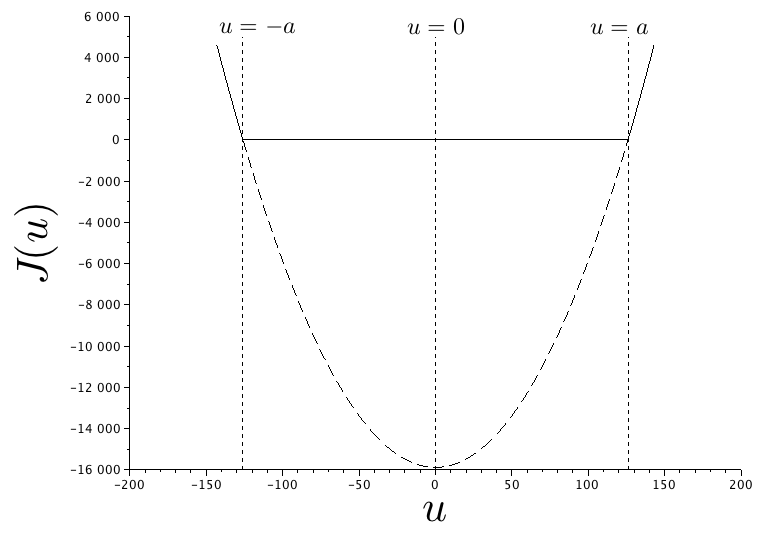
\includegraphics[width=.75\textwidth]{penal_quad.png}
\vspace{-3mm}
\caption{\label{fig:penal_quad} Pénalisation via une parabole tronquée (\cf Eq.~\eqref{eq:penalisation_quad}). }
\end{figure}
Les résultats des optimisations faites avec la pénalisation~\eqref{eq:penalisation_quad} sont présenté dans la Table~\ref{tab:optim2gris_pen_quad}. Ici plus de valeur négative, cependant la borne 1.5 est atteinte à plusieurs reprises. La pénalisation considéré ici n'est que $\mathcal{C}^0$ car il y a 2 points anguleux. Peut-être que cette régularité n'est pas suffisante encore.


Essayons donc une troisième fonction de pénalisation qui est la régularisation de Moreau-Yosida de la pénalisation précédente.
\todo[inline]{Blabla sur la transformée de Moreau Yosida}
La fonction de pénalisation régularisée est alors donnée par :
\begin{equation}
\label{eq:penal_quad_regul}
\mathcal{P}(\tau)=\left\{  \begin{aligned}
0 & \textrm{ si } & E(\tau) - 127.5 \in [ 1.5;253.5 ] \\
\dfrac{1}{2c} ( 126 - E(\tau) )^2 & \textrm{ si } & E(\tau)  \in [-126(2c+1) ; -126 [ \cup ] 126; 126(2c+1) ] \\
\dfrac{(E(\tau))^2}{1+2c}-126^2 & \textrm{ si } & 127.5 < \frac{ E(\tau) }{ 2c+1 }
\end{aligned}  \right.
\end{equation}
\todo[noline]{formulation de la penalisation a revoir}
et est représentée sur la Figure~\ref{fig:penal_quad_regul}. Les niveaux de gris optimaux obtenus avec cette pénalisation sont présentés dans la Table~\ref{tab:optim2gris_pen_quad_reg}.
\begin{figure}
\centering
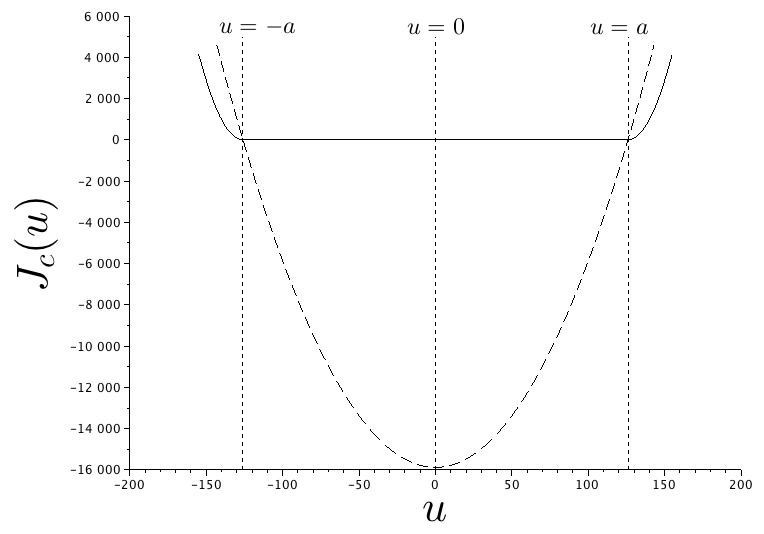
\includegraphics[width=.75\textwidth]{penal_quad_regul.png}
\vspace{-3mm}
\caption{\label{fig:penal_quad_regul} Pénalisation via la régularisation de Moreau-Yosida d'une parabole tronquée (\cf Eq.~\eqref{eq:penal_quad_regul}). }
\end{figure}

Visiblement rien ne semble y faire : il y a toujours des valeurs de $\tau_N$ qui s'approche de 0 et les cas où l'on considère les images $[3,5,7]$ et $[3,7,9]$ fournissent $\tau_N >> \tau_S$ ce qui est aberrant. 
En ce qui concerne l'aberration, cela peut venir du fait que les images 5,7 et 9 sont petites, et donc le bruit est très important et l'image numéro 3, de taille moyenne n'arrive pas à rattraper ce bruit. Il faut donc éviter de prendre en compte les images où la tumeur est trop petite, et si l'on en prend il faut que ces images soient minoritaires devant les autres.

\end{document}